\begin{frame}{Performance in (Unconditional) Protein Generation}
	\begin{center}
		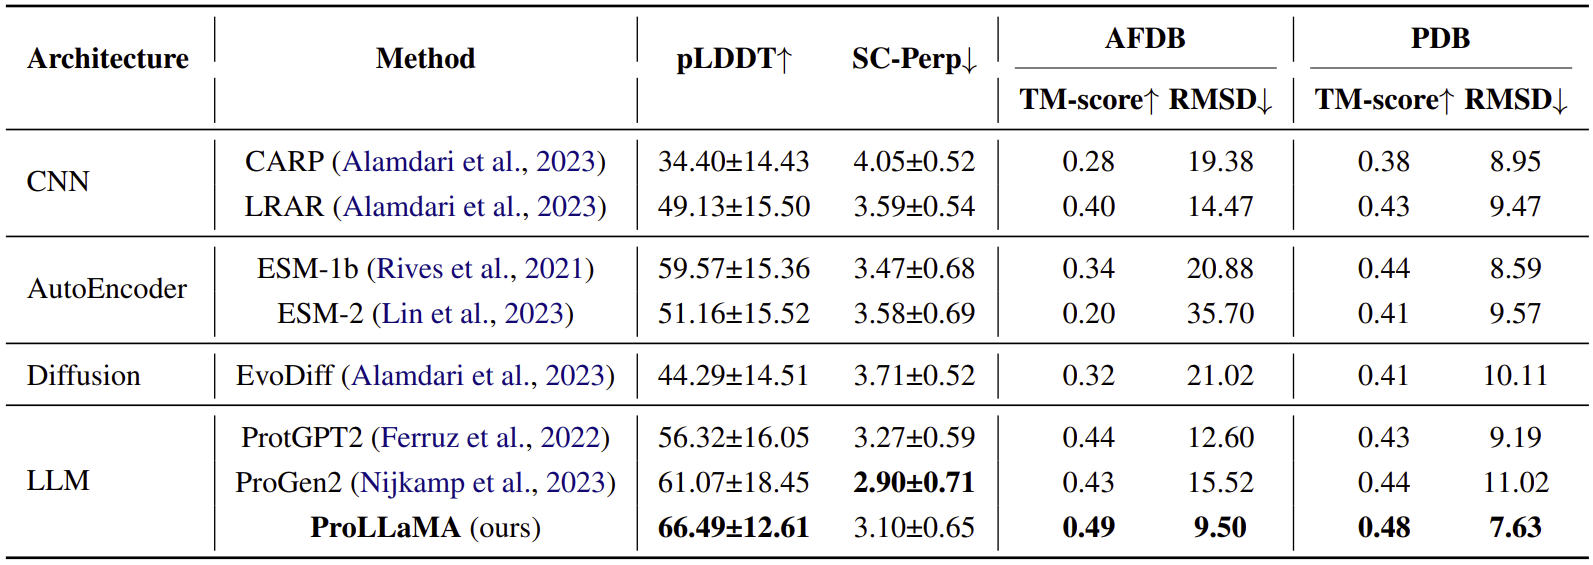
\includegraphics[scale=0.21]{tables/methods_comparison.png}
		\begin{tabular}{>{\centering\arraybackslash}p{11.7em}|>{\centering\arraybackslash}p{3.1em}>{\centering\arraybackslash}p{2.7em}|>{\centering\arraybackslash}p{2.3em}>{\centering\arraybackslash}p{2.3em}|>{\centering\arraybackslash}p{2.3em}>{\centering\arraybackslash}p{2.3em}}
			{\scriptsize \makecell{Natural protein \\ (\cite{alamdari2023protein})}} & \scalebox{.55}{\underline{68.25$\pm$17.85}} & \scalebox{.55}{3.09$\pm$0.63} & & & & \\\hline
		\end{tabular}
		\credit{(Modified) table}{lv2024prollama}
	\end{center}
	%\credit{Table}{lv2024prollama}
	\begin{itemize}
		\item ProLLaMA can generate proteins
		\begin{itemize}
			\item structurally plausible
			\item comparable to natural proteins
		\end{itemize}
	\end{itemize}
\end{frame}